\documentclass{standalone}

\begin{document}

\section[Segmentation]{Image Segmentation}\label{segmentation:unet}

\begin{center}
\begin{figure}[htbp]
\centering
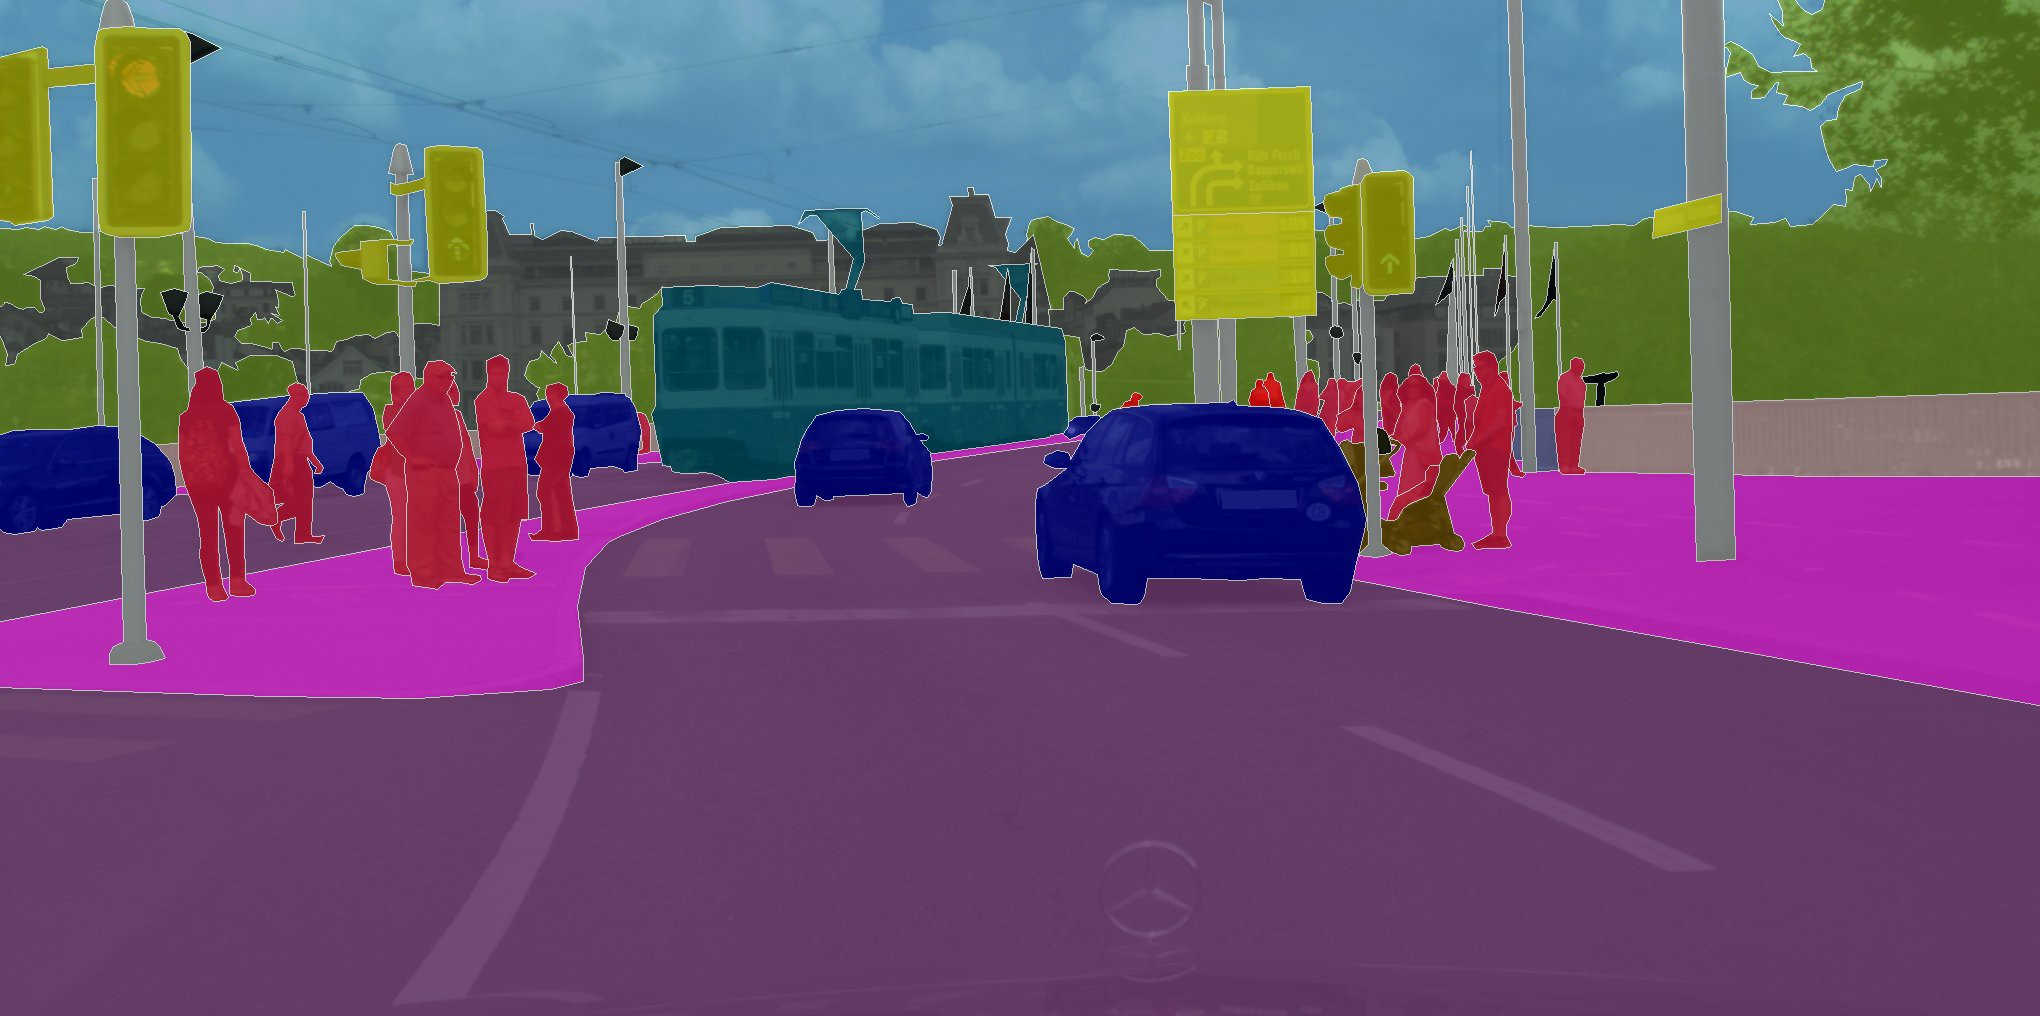
\includegraphics[width=0.85\textwidth]{segmentation.jpg}
\label{fig:segmentation}
\end{figure}
\end{center}

In the previous section we have discussed about object classification and object detection problems (ref.~\ref{obj_detection:obj}).
Now we want to go deeper on this topic, aiming to extract the exact pixels belonging to an object into a given picture.
This kind of problem is called Image Segmentation, i.e give a label to each pixel of the input image.

Image segmentation is a typical task in many research fields and could be used for different purposes.
Information about pixel-wise positions of an object into a picture could be used to extract object shapes or to simplify and/or change the representation of an image into something more meaningful and easier to understand.
This is an hot topic especially for self-driving car applications, where we have to find the exact object shapes to better estimate their perspective position.
All these applications require algorithms fast as much as possible, closed to real-time.

We can face these problems using image processing pipelines or training a Neural Network model.
In the first case, we have to stack a series of functions to process the input image: the pipeline has to filter and extract the useful information about the searched object, but most of all it has to be as most general as possible to face common heterogeneity of image samples.
In the second case, we leave to the Neural Network model parameters the search of the optimal functions combination, but we have to provide a supervised input pattern made by several samples, i.e a combination of inputs and annotated pixel-wise masks of each image.
Image annotation is one of the most hardest and boring steps of image segmentation and for these reasons it is very hard to find public dataset usable.

In this chapter we introduce a Neural Network model commonly used in image segmentation problems, describing its characteristics and performances.
We applied this model to a novel dataset of CT images.
The dataset annotation has been performed using a custom semi-supervised pipeline of image processing developed by the author and the Neural Network model was trained and tested on this dataset.
The original data were taken from \href{https://mrl.sci.utah.edu/software/normal-hip-image-data/}{here}~\cite{doi:10.1002/jor.22040} and the corresponding annotations are released on \href{}{here}. % TODO: add google-drive link

\end{document}
